\documentclass{article}
\usepackage[a4paper,left=3cm, right=3cm, top=2cm, bottom=2cm]{geometry}
\usepackage{amsmath}
\usepackage{graphicx}
\usepackage{caption}
\usepackage{setspace}
\usepackage{xcolor}
\usepackage{titlesec}
\usepackage{amssymb}
\graphicspath{{graph/}}
\title{10.4 Calculus in Polar Coordinates}
\date{}
\author{}
\setstretch{1.2} 

% \subsection* 형식 지정 (번호 없음)
\titleformat{name=\section, numberless}
  {\normalfont\large\bfseries\color{blue}}
  {}
  {0pt}
  {}
\geometry{a4paper, margin=1in}

\begin{document}
\maketitle
This section applies calculus methods to polar curves, focusing on areas, arc lengths, and tangent slopes.

\section*{Area}
To develop the formula for the area A of a region whose boundary is given by a polar equation, we start with the formula for the area of a sector of a circle: $A = \frac{1}{2} r^2\theta$.

Consider a region bounded by a polar curve $r = f(\theta)$ and by rays $\theta = a$ and $\theta = b$. We divide the interval $[a,b]$ into n subintervals of equal width $\Delta\theta$. These rays divide the region into n smaller regions. The area $\Delta A_i$ of the i-th region is approximated by the area of a sector of a circle with radius $f(\theta_i^*)$ and central angle $\Delta\theta$:
\[
\Delta A_i \approx \frac{1}{2} [f(\theta_i^*)]^2 \Delta\theta
\]
Summing these approximations gives a Riemann sum. As $n \to \infty$, this sum approaches the definite integral.
\begin{figure}[htbp]
    \centering
    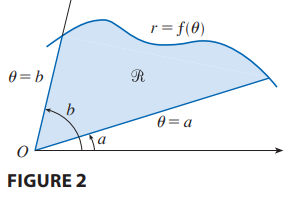
\includegraphics[width=0.3\textwidth]{graph44.png}
    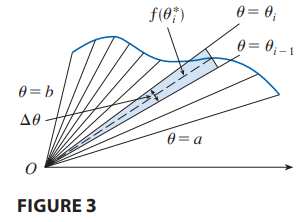
\includegraphics[width=0.3\textwidth]{graph45.png}
\end{figure}

\paragraph{Formula for Area in Polar Coordinates:}
\[
A = \frac{1}{2} \int_{a}^{b} [f(\theta)]^2 \, d\theta \quad \text{or} \quad A = \frac{1}{2} \int_{a}^{b} r^2 \, d\theta
\]

\subsubsection*{EXAMPLE 1}
Find the area enclosed by one loop of the four-leaved rose $r = \cos(2\theta)$.

\paragraph{Solution:} One loop of $r = \cos(2\theta)$ is traced from $\theta = -\pi/4$ to $\theta = \pi/4$. Using symmetry and the area formula:
\[
A = 2 \cdot \frac{1}{2} \int_{0}^{\pi/4} \cos^2(2\theta) \, d\theta
\]
Applying the half-angle identity $\cos^2(u) = \frac{1 + \cos(2u)}{2}$:
\[
A = \int_{0}^{\pi/4} \frac{1 + \cos(4\theta)}{2} \, d\theta = \frac{1}{2} \left[ \theta + \frac{1}{4}\sin(4\theta) \right]_{0}^{\pi/4} = \frac{1}{2} \left( \frac{\pi}{4} \right) = \frac{\pi}{8}
\]

\begin{figure}[htbp]
    \centering
    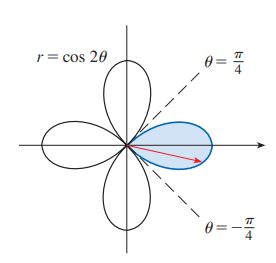
\includegraphics[width=0.33\textwidth]{graph46.png}
\end{figure}

\subsubsection*{EXAMPLE 2}
Find the area of the region inside the circle $r = 3\sin\theta$ and outside the cardioid $r = 1 + \sin\theta$.

\paragraph{Solution:} Intersection points are found by $3\sin\theta = 1 + \sin\theta \implies \sin\theta = 1/2$, yielding $\theta = \pi/6$ and $\theta = 5\pi/6$. The area is the difference of the two areas between these angles:
\begin{align*}
    A &= \frac{1}{2} \int_{\pi/6}^{5\pi/6} \left[ (3\sin\theta)^2 - (1 + \sin\theta)^2 \right] \, d\theta \\
    &= \frac{1}{2} \int_{\pi/6}^{5\pi/6} (9\sin^2\theta - (1 + 2\sin\theta + \sin^2\theta)) \, d\theta \\
    &= \frac{1}{2} \int_{\pi/6}^{5\pi/6} (8\sin^2\theta - 2\sin\theta - 1) \, d\theta
\end{align*}
Using $\sin^2\theta = \frac{1 - \cos(2\theta)}{2}$:
\begin{align*}
    A &= \frac{1}{2} \int_{\pi/6}^{5\pi/6} \left[ 8\left(\frac{1 - \cos(2\theta)}{2}\right) - 2\sin\theta - 1 \right] \, d\theta \\
    &= \frac{1}{2} \int_{\pi/6}^{5\pi/6} (3 - 4\cos(2\theta) - 2\sin\theta) \, d\theta \\
    &= \frac{1}{2} \left[ 3\theta - 2\sin(2\theta) + 2\cos\theta \right]_{\pi/6}^{5\pi/6} = \pi
\end{align*}
\begin{figure}[htbp]
    \centering
    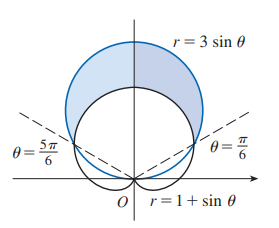
\includegraphics[width=0.32\textwidth]{graph47.png}
\end{figure}

\paragraph{CAUTION:} The fact that a single point has many representations in polar coordinates sometimes makes it dificult to find all the points of intersection of two polar curves. 
\\For instance, it is obvious from picture that the circle and the cardioid have three points of intersection. however, in Example 2 we solved the equations only two such points. The origin is also a point of intersection, but we can’t find it by solving the equations of the curves because the origin has no single representation in polar coordinates that satisfies both equations. 
Notice that, when represented as $(0,0)$ or $(0,\pi)$, the origin satisfies $r = 3 sin\theta $ and so it lies on the circle; when represented as $(0,2/3 \pi)$, it satisfies $r=1+sin\theta$ and so it lies on the cardioid. 
\\Think of two points moving along the curves as the parameter value increases from $0$ to $2\pi$. 
On one curve the origin is reached at $\theta=0$ and $\theta=\pi$ on the other curve it is reached at $\theta=2/3 \pi$.The points don’t collide at the origin because they reach the origin at different times, but the curves intersect there nonetheless.
\\Graphing polar curves is crucial for finding all intersection points. It is especially convenient to use a graphing calculator or computer to help with this task.

\subsubsection*{EXAMPLE 3}
Find all points of intersection of $r = \cos(2\theta)$ and $r = 1/2$.

\paragraph{Solution:} Equating the equations, $\cos(2\theta) = 1/2$, yields $2\theta = \pi/3, 5\pi/3, 7\pi/3, 11\pi/3, \dots$. Thus, for $0 \le \theta < 2\pi$, intersection points are $(1/2, \pi/6)$, $(1/2, 5\pi/6)$, $(1/2, 7\pi/6)$, and $(1/2, 11\pi/6)$.
\begin{figure}[htbp]
    \centering
    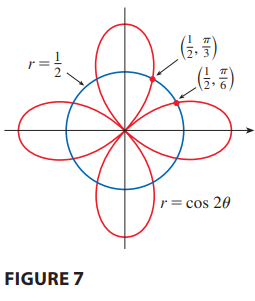
\includegraphics[width=0.3\textwidth]{graph48.png}
\end{figure}

\section*{Arc Length}
To find the length L of a polar curve $r = f(\theta)$ from $\theta = a$ to $\theta = b$, we use its parametric form $x = r\cos\theta$ and $y = r\sin\theta$. Differentiating with respect to $\theta$:
\begin{align*}
    \frac{dx}{d\theta} &= \frac{dr}{d\theta}\cos\theta - r\sin\theta \\
    \frac{dy}{d\theta} &= \frac{dr}{d\theta}\sin\theta + r\cos\theta
\end{align*}
Squaring and summing these gives $\left(\frac{dx}{d\theta}\right)^2 + \left(\frac{dy}{d\theta}\right)^2 = \left(\frac{dr}{d\theta}\right)^2 + r^2$.

\paragraph{Formula for Arc Length in Polar Coordinates:}
\[
L = \int_{a}^{b} \sqrt{r^2 + \left(\frac{dr}{d\theta}\right)^2} \, d\theta
\]

\subsubsection*{EXAMPLE 4}
Find the length of the cardioid $r = 1 + \sin\theta$.

\paragraph{Solution:} The cardioid is traced once for $0 \le \theta \le 2\pi$. With $r = 1 + \sin\theta$, we have $\frac{dr}{d\theta} = \cos\theta$.
\begin{align*}
    L &= \int_{0}^{2\pi} \sqrt{(1 + \sin\theta)^2 + (\cos\theta)^2} \, d\theta \\
    &= \int_{0}^{2\pi} \sqrt{1 + 2\sin\theta + \sin^2\theta + \cos^2\theta} \, d\theta \\
    &= \int_{0}^{2\pi} \sqrt{2 + 2\sin\theta} \, d\theta
\end{align*}
Using the identity $1+\sin\theta = 2\cos^2(\frac{\pi}{4}-\frac{\theta}{2})$ and careful evaluation of the absolute value, the length is 8.

\section*{Tangents}
To find the slope of the tangent line $dy/dx$ to a polar curve $r = f(\theta)$, we use its parametric form.

\paragraph{Formula for Slope of Tangent in Polar Coordinates:}
\[
\frac{dy}{dx} = \frac{\frac{dy}{d\theta}}{\frac{dx}{d\theta}} = \frac{\frac{dr}{d\theta}\sin\theta + r\cos\theta}{\frac{dr}{d\theta}\cos\theta - r\sin\theta}, \quad \text{provided } \frac{dx}{d\theta} \neq 0
\]
Horizontal tangents occur when $\frac{dy}{d\theta} = 0$ (and $\frac{dx}{d\theta} \neq 0$). Vertical tangents occur when $\frac{dx}{d\theta} = 0$ (and $\frac{dy}{d\theta} \neq 0$).

\paragraph{Tangents at the Pole:} If $r = 0$ at $\theta = \theta_0$ and $\frac{dr}{d\theta} \neq 0$, the tangent line at the pole is $\theta = \theta_0$.

\subsubsection*{EXAMPLE 5}
For the cardioid $r = 1 + \sin\theta$: 
\\(a) Find the tangent slope at $\theta = \pi/3$. 
\\(b) Find horizontal and vertical tangent points.

\paragraph{Solution:} Given $r = 1 + \sin\theta$, we have $\frac{dr}{d\theta} = \cos\theta$.
\\(a) At $\theta = \pi/3$, substituting values into the slope formula yields $\frac{dy}{dx} = -1$.\\
(b) Horizontal tangents ($\frac{dy}{d\theta} = 0$): $\cos\theta(1 + 2\sin\theta) = 0$. 
\\This gives $\theta = \pi/2, 3\pi/2, 7\pi/6, 11\pi/6$. The points are $(2, \pi/2)$, $(1/2, 7\pi/6)$, and $(1/2, 11\pi/6)$.

Vertical tangents ($\frac{dx}{d\theta} = 0$): $1 - \sin\theta - 2\sin^2\theta = 0 \implies (1+\sin\theta)(1-2\sin\theta)=0$. 
\\This gives $\theta = 3\pi/2, \pi/6, 5\pi/6$. The points are $(3/2, \pi/6)$ and $(3/2, 5\pi/6)$. At $\theta=3\pi/2$, both derivatives are zero, which corresponds to the cusp at the pole.
\begin{figure}[htbp]
    \centering
    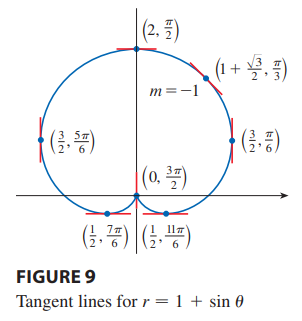
\includegraphics[width=0.35\textwidth]{graph49.png}
\end{figure}

\end{document}
